%%%%%%%%%%%%%%%%%%%%%%%%%%%%%%%%%%%%%%%%%%%%%%%%%%%%%%%%%%%%%%%%%%%%%%%%%%%%%%
\section{Evaluation and Analysis}\label{sec:mtmpi-eva}
%%%%%%%%%%%%%%%%%%%%%%%%%%%%%%%%%%%%%%%%%%%%%%%%%%%%%%%%%%%%%%%%%%%%%%%%%%%%%%

In this section, we evaluate the various techniques designed within
MT-MPI.  All our experiments are executed on the Stam\-pede
supercomputer at the Texas Advanced Computing Center
(https://www.tacc.utexas.edu/stampede/). S\-tampede consists of 6400
Dell Zeus C8220z compute nodes, each with two Xeon E5-2680 processors
and 32~GB RAM, and an Intel Xeon Phi SE10P coprocessor with 8~GB of
on-board RAM connected by an x16 PCIe 2.0 interconnect.  The nodes are
interconnected by a Mellanox FDR InfiniBand network.  All our
experiments are executed on the Xeon Phi coprocessor, with every MPI
process running on a separate coprocessor.


%%%%%%%%%%%%%%%%%%%%%%%%%%%%%%%%%%%%%%%%%%%%%%%%%%%%%%%%%%%%%%%%%%%%%%%%%%%%%%
\subsection{Derived Datatype Processing}\label{sec:eva-ddt}
%%%%%%%%%%%%%%%%%%%%%%%%%%%%%%%%%%%%%%%%%%%%%%%%%%%%%%%%%%%%%%%%%%%%%%%%%%%%%%

In this section, we describe three types of experiments that stress
derived datatype processing to various degrees: (1) derived datatype
packing performance, (2) halo data exchange with derived datatypes,
and (3) the NAS multigrid benchmark. It is noted that we use a similar
for loop for the sequential and parallel version in our comparison. It
allows us to have a fair comparison where both modes are vectorizable,
and both modes have the same issue with prefetching as described in
Section~\ref{sec:imp-ddt}. Thus, the improvement shown will be solely
due to parallelization.

\subsubsection{Derived Datatype Packing}

In our experiments with derived datatype packing (using
\texttt{MPI\_PACK}), we utilized a 3D matrix of doubles, with the X
dimension as the leading dimension.  The matrix volume was fixed at
1~GB, so increasing one dimension would reduce another.  Our
experiments involved packing different 2D planes of the 3D matrix.

\begin{figure}
\begin{center}
\subfigure[Packing the top surface with varying Z dimension.]{
  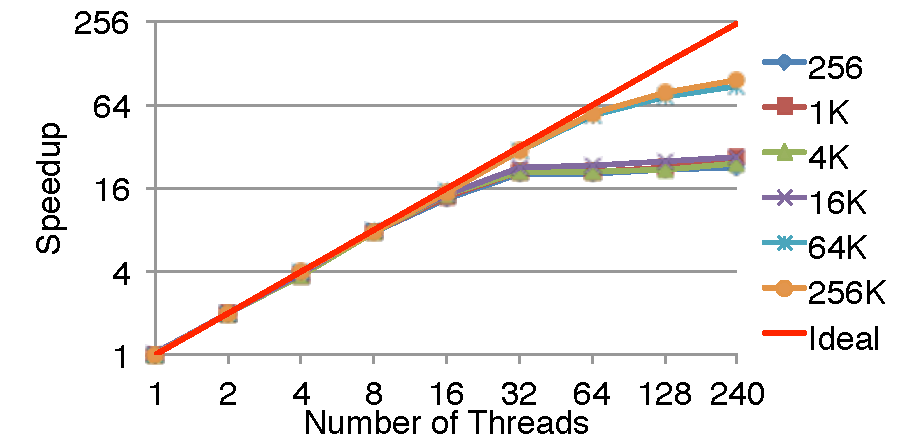
\includegraphics[width=0.8\columnwidth ]{figures/mtmpi/eva-stp-pack-3d-n.pdf}
  \label{fig:eva-pack-3d-n}
}
\subfigure[Packing the left surface with varying Y dimension.]{
  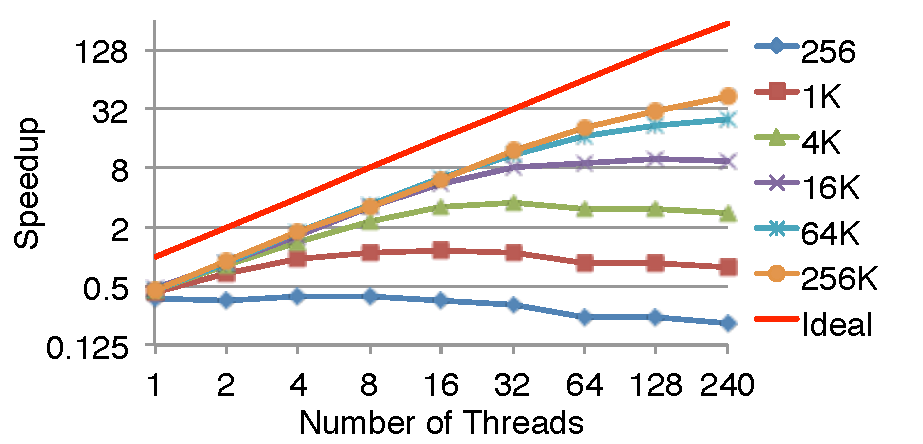
\includegraphics[width=0.8\columnwidth ]{figures/mtmpi/eva-stp-pack-3d-w.pdf}
  \vspace{-2.0ex}
  \label{fig:eva-pack-3d-w}
}
\end{center}
\vspace{-5.0ex}
\caption{Performance of parallel 3D packing.}
\vspace{-3.0ex}
\label{fig:eva-pack-3d}
\end{figure}

Figure~\ref{fig:eva-pack-3d-n} shows the performance improvement while
pac\-king the top surface (X-Z plane).  A vector datatype is utilized in
this case, with a block length equal to the length of the X dimension
and stride equal to the area of the X-Y plane; the Z dimension
indicates the vector count.  In our experiment, the Y dimension was
fixed to 2 doubles, and the Z dimension varied as indicated on the
graph legend (X dimension was varied to maintain the matrix volume).
As can be seen in the figure, MT-MPI gets a reasonably good speedup
with increasing number of threads, achieving a 96-fold improvement
compared with the original sequential version when all 240 threads are
used.  A larger Z dimension provides better speedup because that leads
to a larger iteration count for the contiguous copies and hence more
parallelism that can be exploited by MT-MPI.

Figure~\ref{fig:eva-pack-3d-w} shows the performance improvement while
pac\-king the left surface (Y-Z plane).  A two-level datatype comprising
a vector of vectors is utilized in this experiment.  The X dimension
was fixed to 2 doubles, and the Y dimension varied as indicated on the
graph legend (the Z dimension was varied to maintain the matrix
volume).  As shown in the figure, MT-MPI still achieves a relatively
good speedup compared with the sequential version (42-fold), although
less than what it achieved while packing the top surface.  This
reduction in performance is because the lowest-level vector datatype
always has a block length of one double and a count equal to the Y
dimension.  This restricts the amount of work that is done within each
iteration of the contiguous data copy operation and consequently
limits the work done by each thread, especially when the number of
iterations (i.e., the Y dimension) is small.
%   Furthermore, when the Y
% dimension is small, the parallel version is worse than the original
% sequential version (speedup is less than 1) because of the compiler's
% inefficiency in cache prefetching for vectorized code, as described in
% Section~\ref{sec:imp-ddt}.


\subsubsection{Halo Exchange of Data}

In our second set of experiments, we measured the performance of 3D
halo exchanges of data as used in stencil computations.  Both the data
and the processes are partitioned into a 3D space.  Each process
communicates with its neighboring processes with which it shares a
plane.  For our experiments we define the following four dimension
shapes for the local data on each process: (1) {\tt Cube}, with
dimensions 512 $\times$ 512 $\times$ 512 (doubles); (2) {\tt Large X},
with dimensions 16K $\times$ 128 $\times$ 64; (3) {\tt Large Y}, with
dimensions 64 $\times$ 16K $\times$ 128; and (4) {\tt Large Z}, with
dimensions 64 $\times$ 128 $\times$ 16K.  The MPI processes are evenly
distributed in all dimensions.

Figure~\ref{fig:eva-pack-3d-halo-shapes} shows the performance
improvement achieved by MT-MPI compared with the sequential version
when using 64 MPI processes.  {\tt Large Y} performs much better than
the others, delivering a 23-fold speedup with 240 threads.  To
understand this behavior, we profiled the communication time for the
different dimensions.  The halo benchmark sends data in all dimensions
simultaneously, so it is hard to profile how much time each dimension
takes.  Therefore, for profiling purposes, we modified it to serialize
communication in one dimension at a time, and we observed that
communication along the Y-Z dimension takes 85\% of the time.  While
this is obviously not entirely indicative of the true halo benchmark
that sends data in all dimensions simultaneously, it does give us some
idea of the communication cost.

As demonstrated in Figure~\ref{fig:eva-pack-3d-w}, a large Y dimension
helps improve the performance of packing in the Y-Z dimension by
providing better parallelism.  This results in a large Y impacting the
performance of the halo benchmark to the largest extent.  With {\tt
  Cube}, the Y-dimension is reduced to 512 doubles, thus reducing the
speedup to around 5.8-fold as well.  With {\tt Large X} and {\tt Large
  Z}, the Y-dimension further reduces to 128 doubles, which in turn
reduces the overall speedup to around 1.6-fold and 1.8-fold,
respectively.

\begin{figure}
\begin{center}
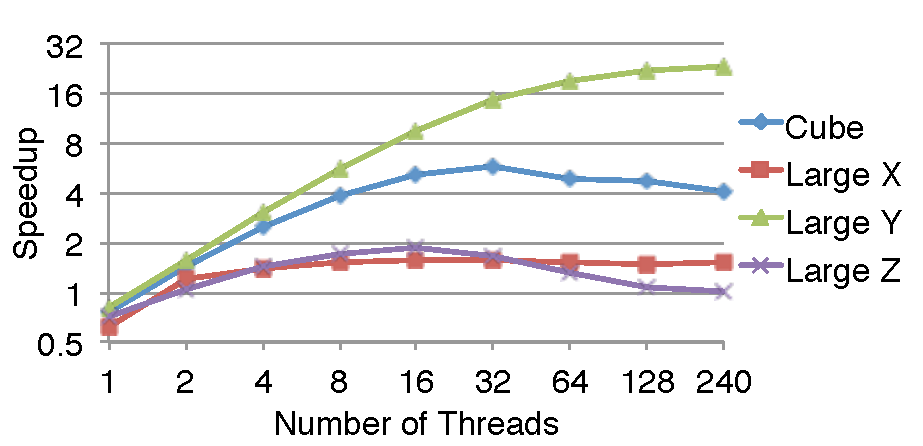
\includegraphics[width=0.8\columnwidth ]{figures/mtmpi/eva-stp-pack-3dhalo-shapes.pdf}
\vspace{-2.0ex}
\caption{3D internode halo exchange using 64 MPI processes.}
\label{fig:eva-pack-3d-halo-shapes}
\end{center}
\vspace{-5.0ex}
\end{figure}

\subsubsection{NAS Multigrid Benchmark}

\begin{figure}[t]
\begin{center}
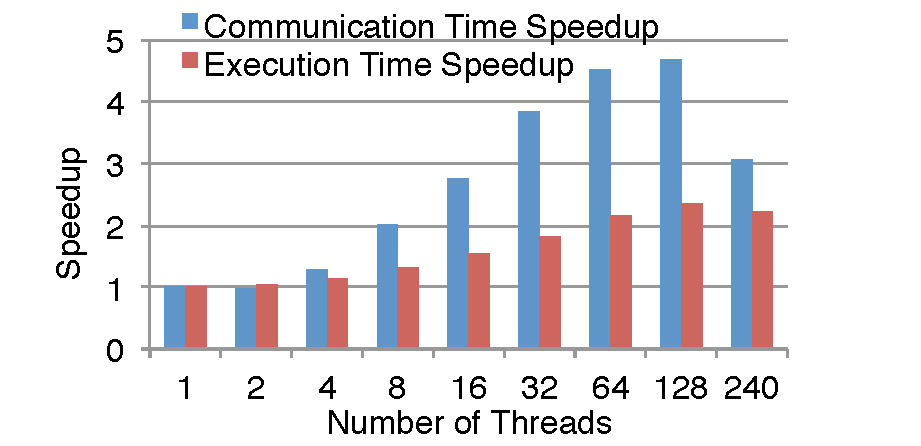
\includegraphics[width=0.8\columnwidth ]{figures/mtmpi/eva-stp-pack-mg-speedup-e.pdf}
\vspace{-2.0ex}
\caption{Hybrid MPI+OpenMP NAS MG Class E using 64 MPI processes.}
\vspace{-5.0ex}
\label{fig:eva-stp-pack-mg-sp-e}
\end{center}
\end{figure}

\begin{figure*}
\begin{center}
\subfigure[Latency.]{
  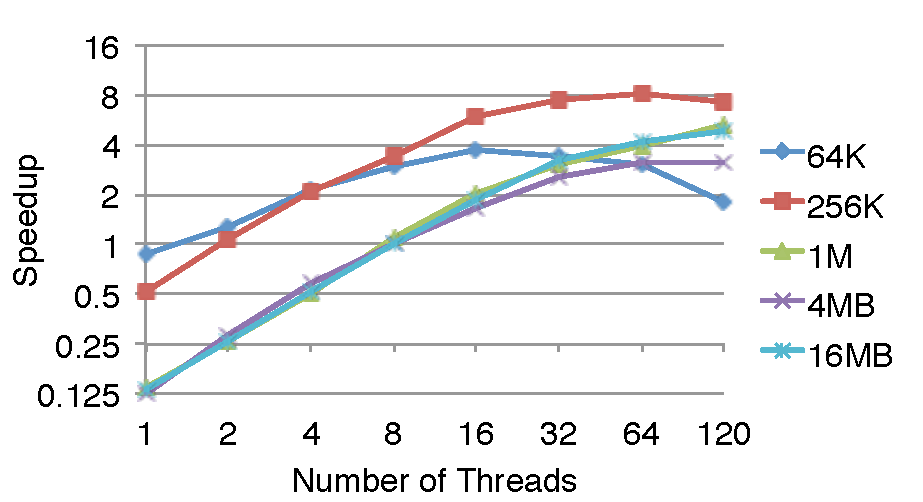
\includegraphics[width=0.63\columnwidth ]{figures/mtmpi/eva-stp-lmt-lat.pdf}
  \label{fig:eva-lmt-2m-latency}
}
\subfigure[Bandwidth.]{
  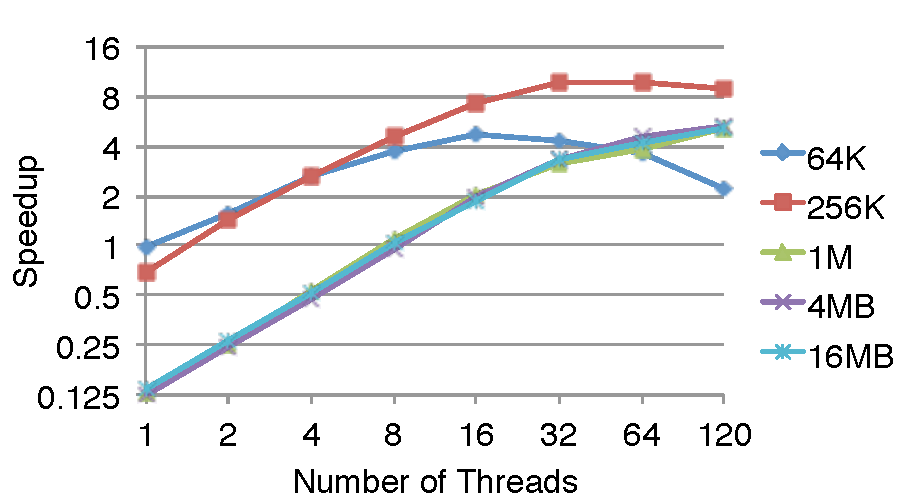
\includegraphics[width=0.63\columnwidth ]{figures/mtmpi/eva-stp-lmt-bw.pdf}
  \label{fig:eva-lmt-2m-bw}
}
\subfigure[Message rate.]{
  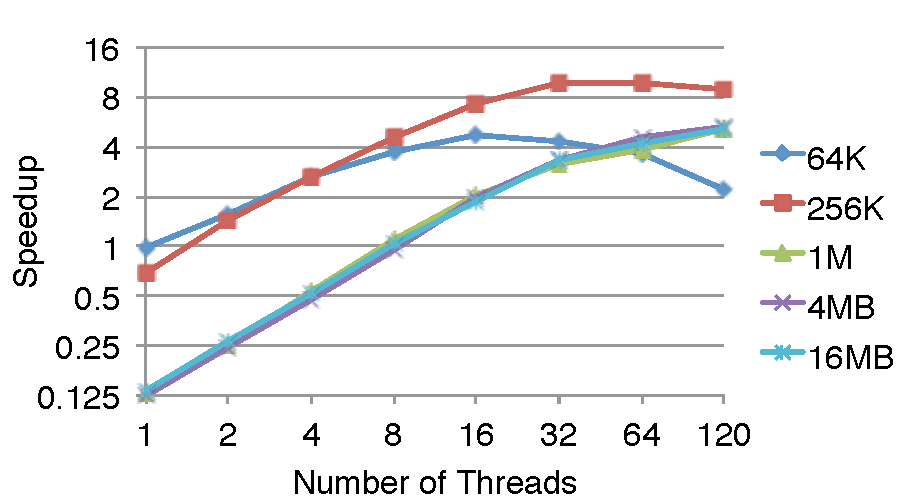
\includegraphics[width=0.63\columnwidth ]{figures/mtmpi/eva-stp-lmt-mr.pdf}
  \label{fig:eva-lmt-2m-mr}
}
\end{center}
\vspace{-5.0ex}
\caption{Shared-memory communication performance with varying message
  size between 2 MPI processes}
\vspace{-3.0ex}
\label{fig:eva-lmt}
\end{figure*}

We also evaluated a hybrid MPI+OpenMP version of the NAS Multigrid
(MG) kernel~\cite{npb} .  The original MG kernel distributed as a part
of the NAS parallel benchmarks does not contain a hybrid MPI+OpenMP
version, so we modified the MPI version to (1) parallelize the local
computation using OpenMP and (2) employ derived datatype communication
instead of manual packing.  The MG kernel implements a V-cycle
multigrid algorithm to solve a 3D discrete Poisson equation.  In every
iteration of the V-cycle routine, halo exchanges are performed with
various dimension sizes (count of double), from 2 to 514 in class E
with 64 MPI processes, and so forth.  The communication in all
dimensions except the X-Y plane is noncontiguous.

Figure~\ref{fig:eva-stp-pack-mg-sp-e} presents the speedup achieved by
MT-MPI compared with the original MPICH in class E (X, Y, Z dimension
sizes are each 2K) when employing 64 processes.  As shown in the
figure, MT-MPI helps improve the communication of MG by 4.7-fold, and
the overall execution time by 2.2-fold.  The speedup in the
communication time is still slightly lower than that of the 3D halo
exchanges with the {\tt Cube} shape shown in
Figure~\ref{fig:eva-pack-3d-halo-shapes}.  The reason is that the MG
also contains some halo exchanges with very small dimension size whose
packing process cannot be parallelized efficiently.


%%%%%%%%%%%%%%%%%%%%%%%%%%%%%%%%%%%%%%%%%%%%%%%%%%%%%%%%%%%%%%%%%%%%%%%%%%%%%%
\subsection{Shared-Memory Communication}\label{sec:eva-lmt}
%%%%%%%%%%%%%%%%%%%%%%%%%%%%%%%%%%%%%%%%%%%%%%%%%%%%%%%%%%%%%%%%%%%%%%%%%%%%%%

To measure the impact of MT-MPI on intranode shared-memory
communication, we evaluated the point-to-point communication benchmarks
in the OSU MPI microbenchmark suite version 4.1
(http://mvapich.cse.ohio-state.edu/benchm\-arks/).  In
particular, we used the latency, bandwidth, and message rate
benchmarks.  Both the original MPICH and MT-MPI use an internal
shared-memory region of 2~MB, with each cell containing 32~KB.

Figure~\ref{fig:eva-lmt} illustrates the performance of all three
benchmarks; the legends in the graph represent different message
sizes.  We notice that the performance trends of all three benchmarks
are similar, with MT-MPI delivering up to a 5-fold performance benefit
for message sizes $\ge$ 1~MB, given enough parallelism.  When the
number of idle threads is $\le$ 4, however, MT-MPI's performance is
worse than that of the original MPICH.  As discussed in
Section~\ref{sec:imp-lmt}, the reason is that MT-MPI loses some of the
pipelining capabilities in the original MPICH code in return for
thread parallelism.  But with a small number of threads, this tradeoff
is not beneficial.

Another observation we make in Figure~\ref{fig:eva-lmt} is that the
speedup of MT-MPI for message sizes 64~KB and 256~KB is much better
than that of other message sizes.  This, however, is not because of
MT-MPI's superior architecture.  Rather, it is because the
communication protocol thresholds (i.e., eager vs. rendezvous
communication thresholds) in MPICH are tuned for regular Xeon systems,
by default, and are too large for the Xeon Phi architecture.  We did
not change the default configuration of MPICH in order to avoid
introducing yet another dimension of variance in the paper.  Thus, for
64~KB and 256~KB message sizes, the original MPICH ends up using a
suboptimal communication protocol, resulting in MT-MPI's performance
falsely appearing to be significantly better as compared to other
message sizes.


%%%%%%%%%%%%%%%%%%%%%%%%%%%%%%%%%%%%%%%%%%%%%%%%%%%%%%%%%%%%%%%%%%%%%%%%%%%%%%
\subsection{InfiniBand Communication Operations}\label{sec:eva-netmod}
%%%%%%%%%%%%%%%%%%%%%%%%%%%%%%%%%%%%%%%%%%%%%%%%%%%%%%%%%%%%%%%%%%%%%%%%%%%%%%

In this section we evaluate the performance benefits achiev\-ed by
MT-MPI with our modifications to the MPICH IB netmod.  We performed two
types of experiments: (1) a one-sided communication microbenchmark
designed to demonstrate the ideal parallelism that can be obtained
within MT-MPI and (2) the one-sided version of Graph500
benchmark~\cite{graph500}.

\subsubsection{One-Sided Microbenchmark}
\label{sec:one-sided-bench}

%GWP - I suggest moving the figure from [t] to next page after fig 10, so perhaps using [h] when you do. Otherwise, fig. 11 comes before fig. 10.
\begin{figure}
\centering
\subfigure[Overall Speedup]{
  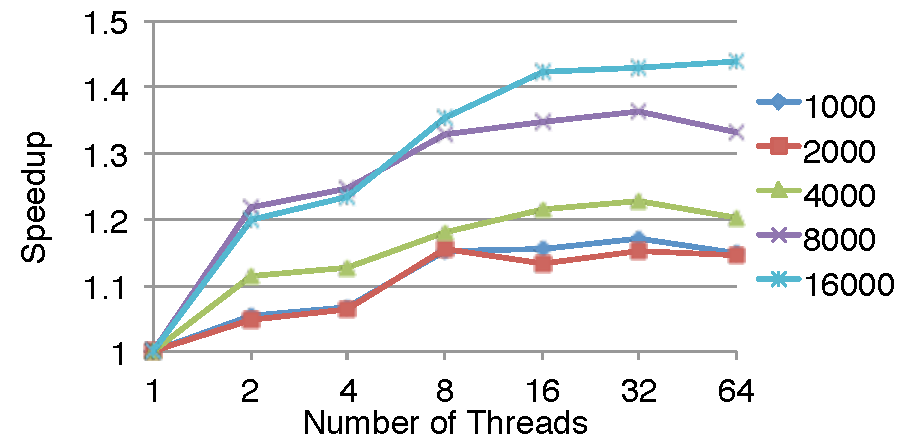
\includegraphics[width=0.8\columnwidth]{figures/mtmpi/eva-stp-ib-one2all.pdf}
  \label{fig:eva-ib-one2all}
}
\subfigure[Send Processing Speedup]{
  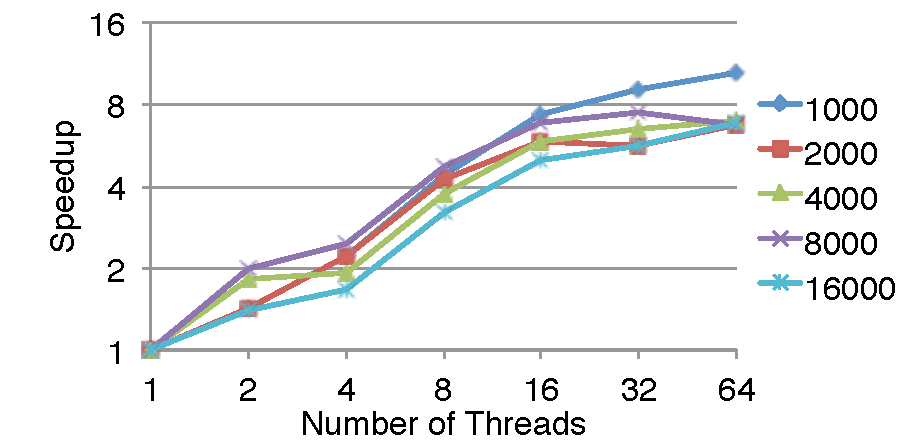
\includegraphics[width=0.8\columnwidth]{figures/mtmpi/eva-stp-ib-one2all-timing.pdf}
  \label{fig:eva-ib-one2all-timing}
}
\vspace{-2.0ex}
\caption{One-sided communication benchmark with IB using 65 MPI processes.}
\vspace{-3.0ex}
\label{fig:eva-ib-micro}
\end{figure}

We designed a microbenchmark in which one MPI process issues many {\tt
  MPI\_PUT} operations to all other processes.  Each \texttt{MPI\_PUT}
operation is for 64 bytes.  We measured the execution time of the
benchmark using 65 MPI processes; thus each process communicates with
64 other processes and internally maintains 64 IB QPs.
Figure~\ref{fig:eva-ib-one2all} shows the speedup in execution time
with MT-MPI compared with the original MPICH.  As we increase the
number of operations issued from 1,000 to 16,000, MT-MPI delivers an
increasing performance benefit, reaching a 1.44-fold speedup when
using 64 threads.

This performance benefit, however, is less than the ideal speedup of
3.1-fold that we can get by parallelizing IB communication, as
discussed in Section~\ref{sec:imp-netmod}.  To understand the reason
for this less-than-ideal speedup, we measured the execution time of
the netmod send-side communication processing at the root process
(SP), which consists only of the copy from the user buffer to a
preregistered chunk and the posting of the operations to the IB
network.  Figure~\ref{fig:eva-ib-one2all-timing} shows that the
execution time of SP delivers around 8-fold speedup when using 64
threads, which is as expected---we expect around a 3.1-fold speedup
due to the parallelization in the posting of network operations, and
some additional improvement due to the parallelized memory copy.
Table~\ref{tab:eva-ib-one2all-timing} shows the relationship between
the time spent in SP and the total execution time when issuing 16,000
operations.  Although SP shows the expected performance improvement
with MT-MPI, the percentage of time spent in SP is less than 10\% when
using more than 16 threads.  This results in a reduction in the
overall performance boost that we achieve.

\begin{table}\scriptsize
\vspace{2.0ex}
\begin{center}
\caption{Profile of the one-sided communication
  benchmark.}\label{tab:eva-ib-one2all-timing}
\vspace{-2.0ex}
\begin{tabular}{|c|ccc|cc|}
\hline
\multirow{2}{*}{Nthreads} &
\multicolumn{3}{c|}{Execution Time} &
\multicolumn{2}{c|}{Speedup} \\
\cline{2-6}
  & Total (s) & SP (s) & SP / Total ({\%}) & Total & SP \\
\hline
1 & 5.8 & 2.2 & 38 & 1 & 1 \\
4 & 4.7 & 1.3 & 27 & 1.2 & 1.7 \\
16 & 4.0 & 0.4 & 10 & 1.4 & 5.0 \\
64 & 4.0 & 0.3 & 8 & 1.4 & 6.9 \\
\hline
\end{tabular}
\end{center}
\vspace{-4.0ex}
\end{table}

\subsubsection{Graph500 Benchmark }

The second benchmark we studied was the Graph500
benc\-hmark~\cite{graph500}, which performs a breadth-first vertex-visit
operation on large graphs.  In particular, we used a scale of $2^{22}$
and an edge factor of 16 on 64 MPI processes running on different
Intel Xeon Phi coprocessors at different nodes.  In the one-sided
version of the Graph500 benchmark, every process issues many {\tt
  MPI\_Accumulate} operations to the other processes in every
breadth-first search iteration.

\begin{figure}
\centering
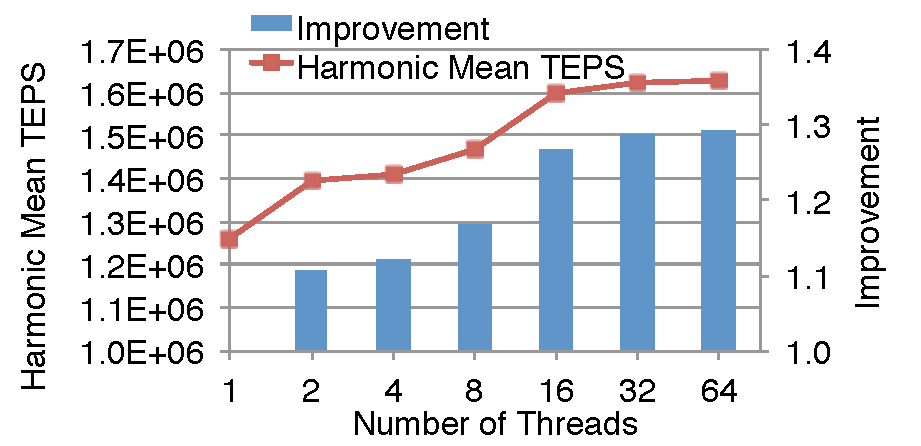
\includegraphics[width=0.8\columnwidth]{figures/mtmpi/eva-stp-ib-graph500.pdf}
\vspace{-2.0ex}
\caption{Performance of the Graph500 benchmark using 64 MPI processes.}\label{fig:eva-graph500-mean-time}
\vspace{-3.0ex}
\end{figure}

Figure~\ref{fig:eva-graph500-mean-time} shows the performance
improvement of MT-MPI compared with the original MPICH.  MT-MPI
delivers a 1.3-fold improvement in the harmonic mean of the traversed
edges per second (TEPS) when using 64 threads.  As expected, this
improvement is on par with the performance improvement we see in the
one-sided communication benchmark that we discussed in
Section~\ref{sec:one-sided-bench}.  The slightly smaller speedup
compared with the one-sided communication benchmark (which achieves a
1.44-fold speedup) is because the Graph500 benchmark does not
uniformly communicate with all peer processes, thus causing some
unevenness in MT-MPI's parallelization.


